
\chapter{Das Haus der Carlsons}
\noindent\textbf{Ort:} Wohnhaus der Carlsons, Arkham, Massachusetts\\
\textbf{Zeit:} 5. April 1920, nach der Unterredung mit Präsident Garmond\\
\textbf{Beteiligte:} Francis Collins, Lillie Johnson, Karim el-Mady, Natheniel Moss

\begin{meisterinfo}
\textbf{Funktion:} Die Ermittler sollen Flynns neun Briefe finden, das Schicksal Helenas erahnen und den Hinweis auf die Universitätsbibliothek mitnehmen. Die Szene ist Ermittlung und übernatürlicher Schrecken, \emph{kein} geplanter Kampf. Die unten angegebenen Probe-Ergebnisse sind Vorschläge; entscheidende Hinweise dürfen nicht an einem einzigen misslungenen Wurf scheitern.

\textbf{Hintergrund:} Die Stimme im Eingangsbereich gehört zu Helena oder einer unheimlichen Wiederholung ihrer Worte. Ein Hrn-Tarl-Ya manifestiert sich im Haus. Die zeitwidrige Alterung des Gebäudes ist eine Folge des Mythosgeschehens. Ungeklärt bleibt bewusst, wie weit die Visionen Vergangenheit zeigen oder die Gegenwart beeinflussen.

\textbf{Handouts:} Neun Briefe an Helena (17.10.1919 bis 20.02.1920); au\ss{}erdem der handschriftliche Bibliothekszettel. Die Briefe werden mit \emph{ihrem tatsächlichen Datum} nummeriert, nicht nach ihrer zufälligen Auffindereihenfolge. Die originale Sammlung liegt als separates Handout vor.
\end{meisterinfo}

\section{2.1 -- Das Haus und sein Grundstück}
\begin{figure}[htbp]\centering
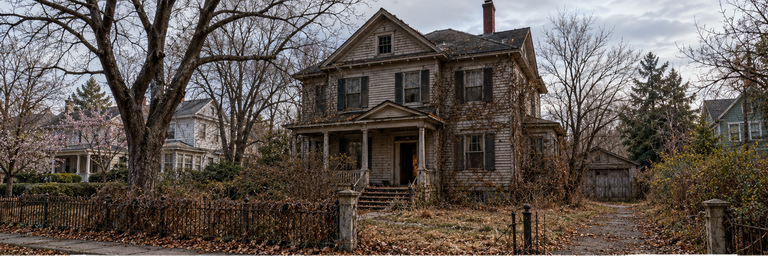
\includegraphics[width=\textwidth]{bilder/carlson-haus-aussen.png}
\caption{Während die Nachbarschaft den Frühling begrü\ss{}t, scheint das Carlson-Grundstück im Winter gefangen.}
\end{figure}
\begin{vorlesetextalle}
Die Adresse führt Euch in eine ruhige Wohnstra\ss{}e am Rande Arkhams. In den Gärten der Nachbarn zeigt sich bereits der Frühling: frische Knospen, saftiges Gras und hier und da das helle Wei\ss{} blühender Obstbäume. Kinderstimmen dringen aus der Ferne herüber, und über einem Zaun hängt frisch gewaschene Wäsche in der Sonne.

Doch das Grundstück, vor dem Ihr stehen bleibt, scheint einer anderen Jahreszeit anzugehören.

Das Haus der Carlsons ist ein gro\ss{}es, zweistöckiges Holzhaus der bürgerlichen Mittelschicht. Unter einem steilen, dunkel gedeckten Dach liegen zwei Reihen hoher Sprossenfenster. Eine überdachte Veranda zieht sich über die Vorderseite. Die einst hell gestrichenen Fassadenbretter sind grau und stumpf; tote Ranken umklammern das Geländer. Zwischen den Zaunlatten haben sich dürre Büsche und Unkraut ausgebreitet. Bis zum Haus führt ein Pfad, auf dem altes Laub in dicken Schichten liegt.

Es ist nicht der verwilderte Garten eines Winters. Es ist ein Grundstück, das aussieht, als sei es seit Jahrzehnten nicht mehr gepflegt worden. Ein paar Schritte weiter, hinter dem Nachbarzaun, blüht ein Strauch in voller Pracht. Hier aber rührt sich kaum ein Blatt.

Hinter den schmutzigen Fensterscheiben ist kein Licht zu erkennen. 
\end{vorlesetextalle}
\begin{meisterinfo}
\textbf{Verborgenes Erkennen (regulär):} Altes, mürbes Laub liegt auch an Stellen, die der Wind normalerweise freifegen würde; frische Triebe fehlen auffällig. Kein Wurf ist nötig, um den Kontrast zur Nachbarschaft zu bemerken. Eine höfliche Befragung der Nachbarn kann ergeben, dass zuletzt kaum jemand Helena gesehen hat; die Nachbarn können keine belastbare Erklärung liefern.
\end{meisterinfo}

\section{2.2 -- Die Veranda und die Stimme}
\begin{vorlesetextalle}
Die Verandadielen geben unter Euren Schritten ein leises, trockenes Knarren von sich. Auf den beiden Schaukelstühlen liegt eine graue Staubschicht. Ein umgekippter Blumentopf hat längst ausgedörrte Erde über die Bretter verteilt. Vor der Haustür sammeln sich verwitterte Blätter.

Die Haustür steht einen schmalen Spalt offen. Durch diesen seht Ihr einen dunklen Flur. Als Ihr klopft oder die Tür vorsichtig bewegt, hört Ihr aus dem Haus eine Frauenstimme:

\glqq{}Kommen Sie herein, ich bin gleich da! Sie können im Wohnzimmer Platz nehmen. Lassen Sie die Schuhe ruhig an.\grqq{}

Schritte entfernen sich in das Innere des Hauses. Dann herrscht wieder Stille.
\end{vorlesetextalle}
\begin{meisterinfo}
\textbf{Stimme:} Niemand erscheint. Wiederholtes Rufen bleibt unbeantwortet; keine zweite klare Ansage. Die Stimme klingt durchaus menschlich. Die Tür darf ohne Probe geöffnet werden. Die Ermittler können sich auch wieder zurückziehen und später zurückkehren.
\end{meisterinfo}

\section{2.3 -- Die Eingangsdiele}
\begin{vorlesetextalle}
Der Flur dahinter ist klein und kühl. Das wenige Tageslicht fällt durch trübe Scheiben auf einen dunkelblauen Teppich, dessen Muster fast im Grau verschwindet. Ein Garderobenschrank mit einigen Mänteln, ein Paar Lederstiefel und ein schmaler Konsolentisch stehen an den Wänden. Vertrocknete Blätter liegen überall auf dem Boden, vermischt mit Erde und Staub. Über einer kleinen Truhe hängt ein fleckiger Spiegel.

Die Luft riecht nach trockenem Holz, kalter Asche und altem Stoff. Seltsam ist die Temperatur: Obwohl drau\ss{}en die Frühlingssonne scheint, ist es hier kälter als im Schatten eines Kellers. Vor Euch führt eine Tür in einen grö\ss{}eren Raum.
\end{vorlesetextalle}
\begin{meisterinfo}
\textbf{Fund -- Brief 1 (17.10.1919):} Auf dem Konsolentisch liegt der erste Brief Flynns, halb unter einer Schale mit ausgetrockneten Blüten. \textbf{Verborgenes Erkennen:} Feine, erdige Abdrücke verlaufen über den Teppich; die Stiefel sind lange nicht getragen worden. Der Brief liegt auf einem etwas helleren, weniger verstaubten Fleck.
\end{meisterinfo}

\section{2.4 -- Der Wohnraum und die erste Vision}
\begin{figure}[htbp]\centering
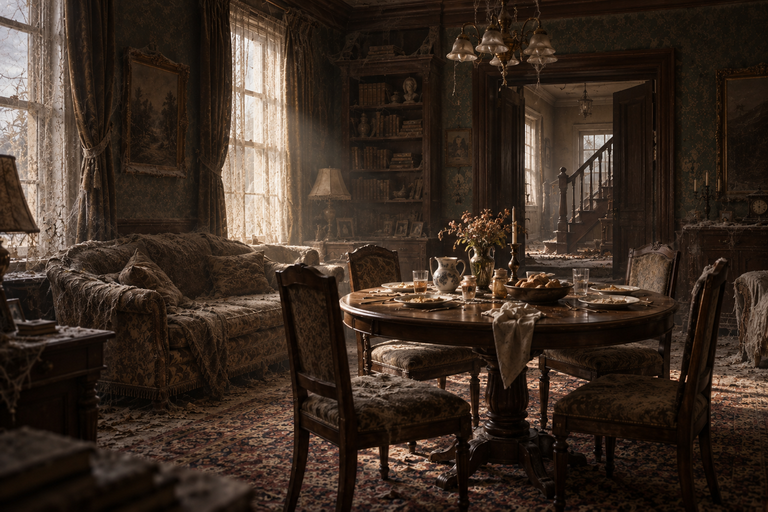
\includegraphics[width=\textwidth]{bilder/carlson-wohnzimmer.png}
\caption{Der Wohnraum: Staub auf Polstern und Möbeln, doch der runde Esstisch wirkt geradezu frisch benutzt.}
\end{figure}
\begin{vorlesetextalle}
Ihr betretet einen geräumigen Wohnraum. Ein Sofa, gepolsterte Sessel, ein Schrank mit Büchern und Porzellan, Bilderrahmen und dunkle Vorhänge zeugen von einer einst behaglichen Einrichtung. Alles ist unversehrt, aber wie unter einem grauen Schleier begraben. Staub liegt auf den Sitzpolstern, auf den Regalen, den Fensterbänken und dem Teppich. Spinnweben hängen an den Vorhangstangen. Man könnte glauben, seit Jahren habe niemand mehr dieses Zimmer betreten.

Nur der gro\ss{}e runde Esstisch in der Mitte widerspricht diesem Eindruck. Seine dunkle Platte ist frei von Staub. Auf ihr stehen Teller, Gläser und eine Karaffe, neben einer Serviette liegen Besteck und die Reste einer Mahlzeit. Es sieht aus, als sei jemand eben erst aufgestanden. Daneben liegen ein kleiner Messingschlüssel, ein ledergebundenes Buch und ein geöffneter Brief.

Eine weitere Tür führt zum hinteren Flur. Aus dieser Richtung dringt kein Laut. Die unnatürliche Stille lässt selbst die kleinsten Geräusche in Euren Ohren widerhallen.
\end{vorlesetextalle}
\begin{meisterinfo}
\textbf{Funde:} Brief 2 (21.10.1919) auf dem Tisch, Brief 3 (05.11.1919) hinter einer gerahmten Fotografie im Schrank. Der Messingschlüssel passt zur Kellertür. Das Lederbuch ist ein unverständlicher Auslöser der Vision; sein Inhalt ist hier nicht zu entziffern. \textbf{Verborgenes Erkennen:} Der Staub entspricht unmöglich nur einer Abwesenheit seit Herbst 1919. \textbf{Naturkunde / Spurensuche:} Feine, ungleichmä\ss{}ige Rillen am Türrahmen deuten nicht auf ein gewöhnliches Werkzeug hin.

\textbf{Auslöser:} Berühren oder bewusstes Untersuchen des Tisches, des Buchs oder der darauf liegenden Gegenstände. Alle Anwesenden werden Zeugen derselben Vision; der Auslöser braucht keine Probe.\end{meisterinfo}
\subsection{Vision I -- Der Verfolger}
\begin{vorlesetextalle}
Im Augenblick der Berührung wird Euch schwindlig. Das fahle Licht des Raumes kippt ins Warme; Staub und Spinnweben sind verschwunden. Ihr steht noch im selben Zimmer, doch die Luft riecht nach Essen und frischer Wäsche. Ihr könnt Euch bewegen, ohne einen Laut zu verursachen, als wärt Ihr blo\ss{}e Zuschauer.

Plötzlich fliegt die Tür zur Diele auf. Eine Frau in einem schlichten Kleid stürzt herein, die Hände an der Brust, den Blick voller Panik über die Schulter geworfen. Ihr Gesicht ist für einen Moment undeutlich wie hinter flie\ss{}endem Glas. Sie taumelt am Tisch vorbei und verschwindet durch die Tür zum hinteren Flur.

Ein Krachen erschüttert den Raum. Die Tür wird aus ihren Angeln gerissen, Holz splittert, und etwas Ungeheuerliches zwängt sich durch die Öffnung. Seine Gliedma\ss{}en sind viel zu lang, seine dunkle Gestalt zieht sich ruckartig zusammen und streckt sich wieder. Finger wie gebogene Klingen fahren über die Wand und rei\ss{}en tiefe Rillen in das Holz. Das Wesen folgt der Frau.

Mitten in der Bewegung hält es inne. Der schmale Kopf dreht sich langsam zurück. Es verharrt, als hätte es ein Geräusch gehört, das in dieser Zeit überhaupt nicht existieren dürfte.

Sein Blick richtet sich genau auf Euch.

Ein schriller, unmenschlicher Laut zerrei\ss{}t die Luft. Dann fällt alles in Dunkelheit. Als Ihr wieder sehen könnt, seid Ihr zurück im grauen Wohnraum. Der Tisch steht noch vor Euch. An der Wand und im Türrahmen zeichnen sich nun tiefe Kratzspuren ab.
\end{vorlesetextalle}
\begin{meisterinfo}
\textbf{Stabilität:} 1/1W4 STA. \textbf{Wichtig:} Das Wesen bemerkt die Beobachter \emph{scheinbar}, kann in der Vision aber nicht bekämpft werden. Die Ermittler werden nicht getrennt. Bei kreativen Versuchen einzugreifen bleibt der Kontakt zu den Gegenständen und zu Helena unwirklich. Die Kratzspuren sind nach der Vision eindeutig vorhanden.
\end{meisterinfo}

\subsection{Das Wesen in der Vision}
\begin{figure}[htbp]\centering
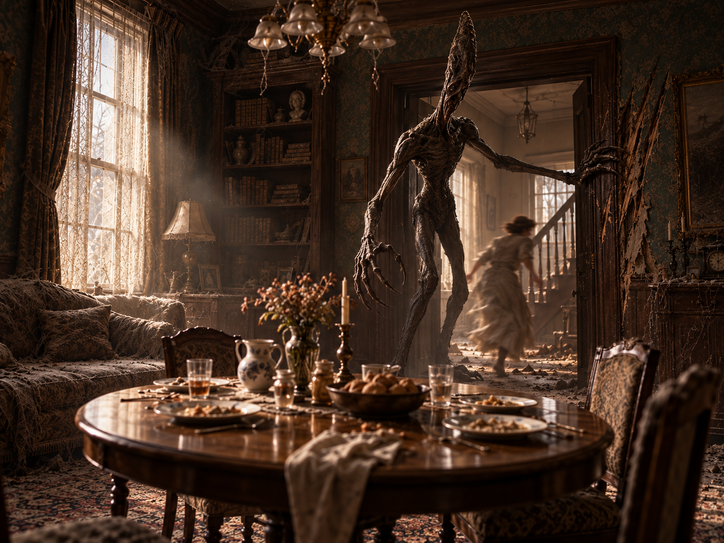
\includegraphics[width=0.95\textwidth]{bilder/gnicht-tyaacht-vision.png}
\caption{So könnte das Hrn-Tarl-Ya in der ersten Vision auf die Ermittler gewirkt haben.}
\end{figure}
\begin{meisterinfo}
\textbf{Erscheinungsbild:} Das Hrn-Tarl-Ya wirkt wie ein unnatürlich hochgewachsener, aus Holz, Haut und Schatten zusammengeflickter Verfolger. Seine Gliedma\ss{}en sind zu lang, die Bewegungen ruckartig und schnell, der Kopf schmal und fremdartig. Nutze die Illustration zur atmosphärischen Einordnung; die Spieler sollten das Wesen nicht lange und nie vollständig betrachten können.
\end{meisterinfo}

\section{2.5 -- Hinterer Flur und Treppenhaus}
\begin{vorlesetextalle}
Die zweite Tür führt in einen schmalen Flur. Eine Holztreppe steigt in das Obergeschoss hinauf, daneben liegt der Zugang zur Küche. Unter den Stufen befindet sich eine niedrige Tür. Über den Dielen liegt derselbe graue Film wie im übrigen Haus; ein verblasster Läufer ist an den Rändern steif geworden. An der Wand hängt schief ein Familienbild.

Auf dem Treppengeländer ziehen sich lange, unregelmä\ss{}ige Furchen nach oben. Ihr habt das Gefühl, dass sich die Kälte hier sammelt.
\end{vorlesetextalle}
\begin{meisterinfo}
Die Kellertür liegt unter der Treppe und ist verschlossen. Der Messingschlüssel aus dem Wohnzimmer öffnet sie. Andere Wege sind \emph{Schlosser} oder eine passende Kraftprobe; ein Fehlschlag kann Zeit oder Lärm kosten, darf die Erkundung aber nicht blockieren. Das Familienbild zeigt Flynn und Helena.
\end{meisterinfo}

\section{2.6 -- Die Küche}
\begin{vorlesetextalle}
In der Küche stehen ein gusseiserner Herd, eine Spüle und schwere Holzschränke. Auf einer Arbeitsplatte liegen ein Hackbrett und ein Messer; daneben stapelt sich ungewaschenes Geschirr. In einer Ecke ist ein kleiner Tisch teilweise mit einem verblichenen Tuch bedeckt. Eine umgesto\ss{}ene Schüssel hat vertrocknete Speisereste über die Dielen verteilt.

Auch hier ruht dicker Staub auf allem. An den Fenstern sitzt ein milchiger Beschlag, und der Atem scheint beim Sprechen fast sichtbar zu werden. In der Nähe des Herdes ist die vermeintliche Staubschicht nicht grau, sondern hell und kristallin.
\end{vorlesetextalle}
\begin{meisterinfo}
\textbf{Fund -- Brief 4 (22.11.1919):} In einer Schublade zwischen Tüchern. \textbf{Verborgenes Erkennen:} Was auf dem Herdrand wie Staub wirkt, ist feiner Reif. \textbf{Horchen:} Gelegentlich ein leises Kratzen, schwer zu orten, doch es scheint nicht aus den Wasserrohren zu stammen.
\end{meisterinfo}

\section{2.7 -- Der Keller}
\begin{vorlesetextalle}
Hinter der niedrigen Tür führt eine steile Holztreppe hinunter. Jeder Tritt gibt ein dumpfes Ächzen von sich. Die Luft wird schwer und erdig. Eine Laterne erhellt Kohlenvorräte, Regale mit Gläsern, Vorratskisten und einen alten Waschtrog.

In einer Ecke liegt eine Decke auf dem Boden. Daneben stehen ein fast leerer Wasserkrug und eine Petroleumlampe. Es sieht aus, als habe jemand sich hier versteckt. Innen an der Tür verlaufen mehrere tiefe, dicht beieinanderliegende Furchen. Die Holzsplitter zeigen in den Keller hinein.
\end{vorlesetextalle}
\begin{meisterinfo}
\textbf{Fund -- Brief 5 (17.12.1919):} In einer Blechdose unter der Decke. \textbf{Zusatzfund (optional):} Ein Zettel in Helenas Handschrift: \glqq{}Es kann Stimmen nachmachen. Ich höre es oben gehen.\grqq{} Diese Notiz ist \emph{neu} und gehört nicht zu den ursprünglichen Handouts. \textbf{Verborgenes Erkennen:} Ein Streifen lockerer Erde führt zu einer Ritze im Mauerwerk und endet dort ohne erkennbare Fortsetzung.
\end{meisterinfo}

\section{2.8 -- Gang im Obergeschoss}
\begin{vorlesetextalle}
Die Treppe mündet in einen schmalen, dunkleren Gang. Hier oben ist es noch kälter als unten. Durch die trüben Fenster fällt nur wenig Licht; an den Türgriffen hängt Staub wie eine zweite Patina. Drei Zimmertüren gehen vom Flur ab. Am Ende steigt eine schmale Holzstiege zu einer Luke unter dem Dach hinauf.
\end{vorlesetextalle}
\begin{meisterinfo}
Der Gang verbindet Schlafzimmer, Bad und früheres Gästezimmer beziehungsweise Lager. Wer länger lauscht, hört möglicherweise einmal trockenes Knacken über dem Kopf. Die Stiege zum Dachboden ist frei zugänglich.
\end{meisterinfo}

\section{2.9 -- Schlafzimmer}
\begin{vorlesetextalle}
Ein breites Bett mit sorgfältig gezogener Tagesdecke füllt den Raum. Zwei Nachttische, ein Kleiderschrank und eine Kommode stehen an den Wänden. Auf einer Spiegelablage liegen Bürste und Haarnadeln, daneben befindet sich ein gerahmtes Foto des Ehepaars. Flynns Kleidung hängt noch im Schrank, Helenas Kleider daneben.

Die Gegenstände erzählen von einem bewohnten Haus, das plötzlich verlassen wurde. Doch der Staub auf den Bettdecken scheint aus einer anderen Zeit zu stammen.
\end{vorlesetextalle}
\begin{meisterinfo}
\textbf{Fund -- Brief 6 (05.01.1920):} In der obersten Kommodenschublade. \textbf{Verborgenes Erkennen:} Kein Koffer fehlt, kein Reisekleid liegt bereit. Weitere Familienbilder sind vorhanden. Keine Probe ist nötig, um das Fehlen von Anzeichen einer geplanten Abreise zu erkennen.
\end{meisterinfo}

\section{2.10 -- Bad}
\begin{vorlesetextalle}
Das Bad ist klein, mit freistehender Wanne, Waschbecken und schmalem Spiegelschrank. Die Porzellanschalen sind stumpf, die Armaturen angelaufen. Auf dem Waschtisch stehen halb leere Fläschchen und eine Seifendose. Das Fenster ist von einem grauen Film überzogen. Ein Tropfen fällt irgendwo in das Waschbecken, doch die Leitung scheint trocken zu sein.
\end{vorlesetextalle}
\begin{meisterinfo}
\textbf{Fund -- Brief 7 (12.01.1920):} Gefaltet hinter den Fläschchen im Spiegelschrank. \textbf{Optionaler Gruseleffekt:} Ein Ermittler glaubt im Spiegel eine Gestalt hinter sich zu sehen; beim Umdrehen ist niemand dort. Keine Stabilitätsprobe, solange der Eindruck flüchtig bleibt.
\end{meisterinfo}

\section{2.11 -- Gäste- und Lagerzimmer}
\begin{vorlesetextalle}
Hier stehen unter fleckigen Leinentüchern kleine Möbel, ein alter Paravent, Hutschachteln und mehrere gestapelte Holzkisten. An einer Wand lehnt ein schmales Kinderbett ohne Matratze, offenbar lange nicht benutzt. Die Luft ist stickig, und bei jeder Bewegung wirbeln graue Flocken auf.
\end{vorlesetextalle}
\begin{meisterinfo}
\textbf{Fund -- Brief 8 (07.02.1920):} Zwischen alten Papieren in einer Hutschachtel. \textbf{Verborgenes Erkennen:} Eine Spur durch die Staubschicht läuft an der Wand entlang und endet abrupt über Bodenhöhe; sie ist mit menschlichen Schritten nicht leicht zu erklären.
\end{meisterinfo}

\section{2.12 -- Dachboden, letzter Brief und Bibliothekshinweis}
\begin{vorlesetextalle}
Die schmale Stiege endet unter einer Dachluke. Darüber liegt ein niedriger Dachboden, durchzogen von schweren Balken und unterbrochen von alten Truhen, Koffern und Möbelteilen. Ein kleines rundes Dachfenster lässt nur einen trüben Lichtfleck herein. Die Luft ist trocken und bei\ss{}end, und selbst das Knarren des Holzes scheint hier oben gedämpft.

An einem hohen Querbalken bewegt sich etwas kaum merklich im Luftzug. Zwischen zwei alten Kisten liegt eine schmale Mappe mit Papieren.
\end{vorlesetextalle}
\begin{meisterinfo}
\textbf{Funde:} Brief 9 (20.02.1920) in der Mappe; daneben der originale Handout-Zettel \glqq{}Archäologie in Ägypten von M. Dyers, 1899 -- Bücherei an der Miskatonic Universität -- EB8/II-474\grqq{}. Der Zettel führt unmittelbar zu Szene 3. \textbf{Verborgenes Erkennen:} Ein Seil verschwindet im Dämmerlicht über einem Balken; an ihm sind deutliche Scheuerstellen. Den Ermittlern darf die dunkle Gestalt zunächst entgehen, bis sie sich nähern oder mehr Licht schaffen.

\textbf{Räumliche Festlegung:} Die Erhängte befindet sich \emph{im Dachboden} unter dem Dach, nicht auf der gefährlichen Au\ss{}enseite des Dachs. Das entspricht der älteren Meisterskizze und erlaubt die geplante Lichtveränderung durch das Dachfenster.\end{meisterinfo}

\section{2.13 -- Helena Carlson: die zweite Vision}
\begin{vorlesetextalle}
Erst als Ihr Euch an die Schatten unter den Balken gewöhnt, erkennt Ihr, was dort hängt. Es ist eine Frau in einem schlichten Kleid. Ihr Körper schwebt reglos wenige Fingerbreit über den staubigen Dielen. Das Gesicht ist im Halbdunkel kaum zu erkennen, die Arme hängen schlaff herab.
\end{vorlesetextalle}
\begin{meisterinfo}
\textbf{Auslöser:} Berührung der Frau oder des Seils. Die Vision tritt für alle Anwesenden ein, die sich auf dem Dachboden befinden. Falls niemand die Gestalt berührt, kann das Licht bei einem vorsichtigen Untersuchungsversuch ebenfalls umschlagen. \textbf{Stabilität:} Beim Auffinden des Leichnams 0/1W3, bei der folgenden Vision 1/1W6 (Spielleiterentscheidung, kumulative Belastung beachten).
\end{meisterinfo}
\begin{vorlesetextalle}
In dem Augenblick, in dem Ihr den Körper berührt, verändert sich das Licht. Eben noch fiel nur ein trüber Schein durch das verschmutzte Dachfenster. Jetzt strömt helles Sonnenlicht herein, als wäre das Glas mit einem Schlag klar geworden. Die staubigen Balken leuchten goldbraun.

Die Frau hebt den Kopf. Ihre Augen sind geöffnet. Sie sieht Euch an, nicht mit blindem Schrecken, sondern mit einem schmerzlichen, dringlichen Blick. Langsam hebt sie ihren rechten Arm und streckt Euch die Hand entgegen.

\glqq{}Findet meinen Mann.\grqq{}

Ihre Lippen zittern.

\glqq{}Findet Flynn. Bitte ... rettet ihn.\grqq{}

Dann erlischt das Licht wie eine Kerze im Wind. Alles wird wieder grau. Das Seil schwingt leicht über Euch -- aber die Frau ist fort. Kein Körper liegt am Boden, kein Geräusch verrät, wohin sie verschwunden sein könnte.
\end{vorlesetextalle}

\section{2.14 -- Das Wesen im Haus}
\begin{vorlesetextalle}
Aus den unteren Stockwerken dringt ein Schrei, der nicht menschlich sein kann. Er beginnt tief und heiser, steigt in eine schneidende Höhe und bricht unvermittelt ab.

Danach hört Ihr Kratzen. Langsame, schwere Schläge gegen Holz, als würden lange Krallen an den Wänden entlangziehen. Das Geräusch bewegt sich unter Euch durch das Haus.

Wer vorsichtig durch die Dachbodenluke schaut, sieht im Halbdunkel des Ganges einen viel zu langen Arm, eine schmale Schulter und einen Kopf, der sich ruckartig bewegt. Dann verschwindet die Gestalt hinter der Treppenbiegung. Das Kratzen entfernt sich langsam.
\end{vorlesetextalle}
\begin{meisterinfo}
\textbf{Ziel:} Die Gefahr soll überwältigend wirken, aber keine zwangsläufige tödliche Falle darstellen. \textbf{Schleichen / Horchen:} Bei Gelingen erkennen die Ermittler eine günstige Pause und können sich leise zurückziehen. Bei einem Fehlschlag rückt das Kratzen näher oder eine Tür schlägt; es folgt nicht automatisch ein tödlicher Angriff. \textbf{Verhalten:} Warten, leise bleiben, dann gemeinsam das Haus verlassen. Wer aktiv gegen das Wesen vorgeht, erlebt seine erschreckende Überlegenheit; die konkreten Werte werden erst bei einer tatsächlichen Konfrontation benötigt.
\end{meisterinfo}

\subsection{Spielwerte des Hrn-Tarl-Ya}
\begin{figure}[htbp]\centering
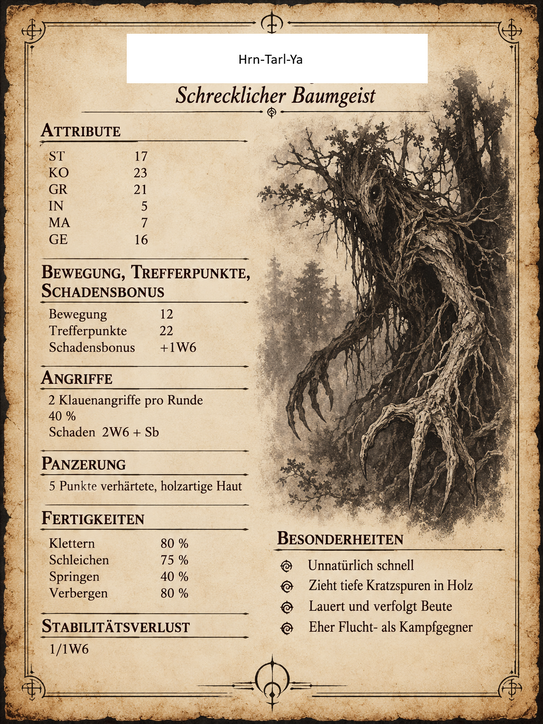
\includegraphics[width=0.82\textwidth]{bilder/gnicht-tyaacht-statblock.png}
\caption{Spielwerte des Hrn-Tarl-Ya für die Spielleitung.}
\end{figure}
\begin{meisterinfo}
\textbf{Einsatz im Abenteuer:} Diese Werte sind als Sicherheitsnetz für die Spielleitung gedacht. Das Wesen ist im Carlson-Haus in erster Linie ein Schrecken aus der Peripherie -- ein Verfolger, vor dem man flieht, nicht ein fairer Kampfgegner. Setze es sparsam ein: andeuten, hören lassen, kurz sehen lassen, Rückzug ermöglichen.

\textbf{Regelhinweis:} Der Stat-Block basiert auf Euren alten Unterlagen zum Hrn-Tarl-Ya und ist für die Szene leicht zugespitzt: zwei Klauenangriffe pro Runde, zähe holzartige Haut und hohe Werte in Schleichen, Klettern und Verbergen. Wenn Ihr die Szene rein erzählerisch halten wollt, reichen die Angaben im Flie\ss{}text bereits aus.
\end{meisterinfo}

\section{2.15 -- Flucht und Übergang zur Bibliothek}
\begin{vorlesetextalle}
Als Ihr endlich die Haustür hinter Euch lasst, weht Euch der warme Frühlingswind entgegen. In der Stra\ss{}e ist nichts verändert. Ein Vogel ruft, hinter dem Zaun des Nachbarn klappert Geschirr, und an einem Baum öffnen sich junge Blätter.

Das Haus der Carlsons steht grau und reglos hinter Euch. Sein Garten zeigt kein einziges Zeichen des Frühlings. Die Haustür bleibt einen schmalen Spalt offen.
\end{vorlesetextalle}
\begin{meisterinfo}
\textbf{Szenenergebnis:} Die Briefe dokumentieren Flynns Reise und den Zusammenbruch der Expedition. Helenas Vision bittet ausdrücklich darum, Flynn zu retten. Der Zettel mit dem Buchtitel und der Signatur führt die Gruppe in die Universitätsbibliothek. \textbf{Ausfallsicherung:} Werden Briefe übersehen, kann die Mappe auf dem Dachboden mehrere davon enthalten; der Bibliothekszettel sollte keinesfalls unauffindbar bleiben. \textbf{Nächste Szene:} Akt I, Szene 3 -- Das Geheimnis der Universitätsbibliothek.
\end{meisterinfo}
